\begingroup
\definecolor{tradeink}{HTML}{17293C}
\definecolor{tradelight}{HTML}{F0F4F7}
\definecolor{tradeborder}{HTML}{C3CFD8}
\definecolor{tradeblue}{HTML}{486E91}
\definecolor{tradegreen}{HTML}{196D60}
\definecolor{tradeamber}{HTML}{AD6229}
\resizebox{\linewidth}{!}{%
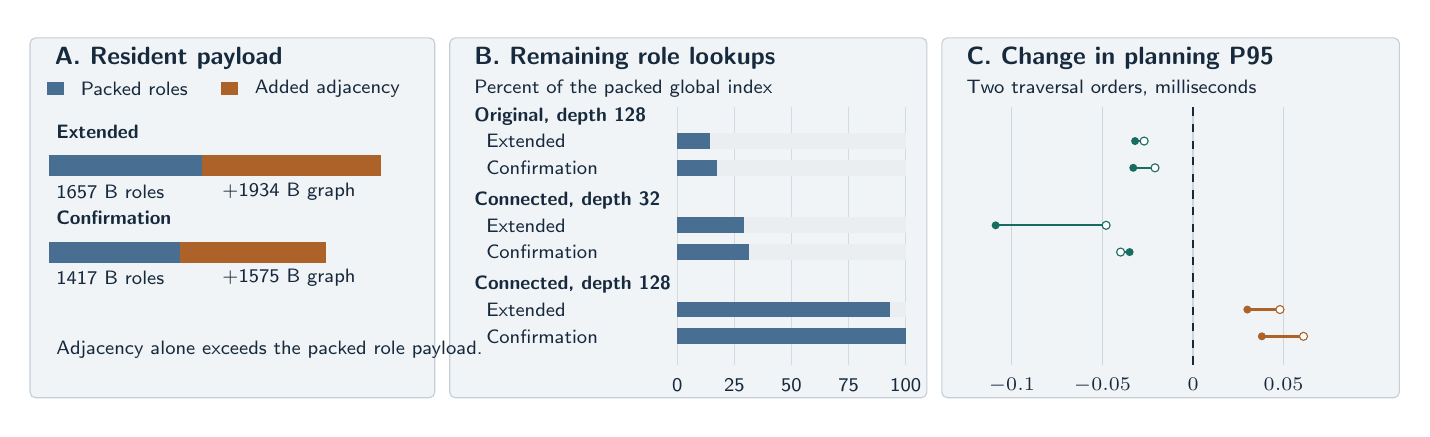
\begin{tikzpicture}[x=1cm,y=1cm,color=tradeink,font=\sffamily\scriptsize,
  heading/.style={font=\sffamily\small\bfseries,anchor=west},
  frame/.style={rounded corners=2pt,draw=tradeborder,fill=tradelight}]
  \path[use as bounding box] (0,0) rectangle (17.45,4.84);
  \draw[frame] (.03,.14) rectangle (5.17,4.71);
  \draw[frame] (5.36,.14) rectangle (11.42,4.71);
  \draw[frame] (11.61,.14) rectangle (17.42,4.71);
  \node[heading] at (.22,4.45) {A. Resident payload};
  \node[heading] at (5.55,4.45) {B. Remaining role lookups};
  \node[heading] at (11.80,4.45) {C. Change in planning P95};

  \fill[tradeblue] (.24,3.98) rectangle (.46,4.15);
  \node[anchor=west] at (.55,4.06) {Packed roles};
  \fill[tradeamber] (2.45,3.98) rectangle (2.67,4.15);
  \node[anchor=west] at (2.76,4.06) {Added adjacency};
  \foreach \desc/\y/\r/\m in {Extended/3.22/1657/1934,Confirmation/2.12/1417/1575} {
    \node[anchor=west,font=\sffamily\bfseries\scriptsize] at (.24,{\y+.30}) {\desc};
    \fill[tradeblue] (.27,{\y-.27}) rectangle ({.27+.00118*\r},\y);
    \fill[tradeamber] ({.27+.00118*\r},{\y-.27}) rectangle ({.27+.00118*(\r+\m)},\y);
    \node[anchor=west] at (.24,{\y-.46}) {\r\ B roles};
    \node[anchor=west] at (2.35,{\y-.46}) {+\m\ B graph};
  }
  \node[anchor=west,align=left] at (.24,.75) {Adjacency alone exceeds\ the packed role payload.};

  \node[anchor=west] at (5.55,4.07) {Percent of the packed global index};
  \node[anchor=west] at (11.80,4.07) {Two traversal orders, milliseconds};
  \foreach \v in {0,25,50,75,100} {
    \draw[tradeborder!75] ({8.25+.029*\v},.56) -- ({8.25+.029*\v},3.83);
    \node[anchor=north] at ({8.25+.029*\v},.51) {\v};
  }
  \foreach \d in {-.10,-.05,0,.05} {
    \draw[tradeborder!85] ({12.04+23*(\d+.12)},.56) -- ({12.04+23*(\d+.12)},3.83);
    \node[anchor=north] at ({12.04+23*(\d+.12)},.51) {\pgfmathprintnumber[fixed,precision=2]{\d}};
  }
  \draw[tradeink,dashed] ({12.04+23*.12},.56) -- ({12.04+23*.12},3.83);
  \node[anchor=west,font=\sffamily\bfseries\scriptsize] at (5.55,3.71) {Original, depth 128};
  \node[anchor=west,font=\sffamily\bfseries\scriptsize] at (5.55,2.64) {Connected, depth 32};
  \node[anchor=west,font=\sffamily\bfseries\scriptsize] at (5.55,1.57) {Connected, depth 128};

  \foreach \desc/\y/\pct/\a/\b in {
    Extended/3.40/14.2/-.032/-.027,
    Confirmation/3.06/17.6/-.033/-.021,
    Extended/2.33/29.3/-.109/-.048,
    Confirmation/1.99/31.4/-.035/-.040,
    Extended/1.26/93.3/.030/.048,
    Confirmation/.92/100/.038/.061}
  {
    \node[anchor=west] at (5.70,\y) {\desc};
    \fill[tradeborder!35] (8.25,{\y-.10}) rectangle (11.15,{\y+.10});
    \fill[tradeblue] (8.25,{\y-.10}) rectangle ({8.25+.029*\pct},{\y+.10});
    \pgfmathtruncatemacro{\slower}{\a>0}
    \ifnum\slower=1 \def\effectcolor{tradeamber}\else \def\effectcolor{tradegreen}\fi
    \draw[\effectcolor,line width=.85pt] ({12.04+23*(\a+.12)},\y)
          -- ({12.04+23*(\b+.12)},\y);
    \fill[\effectcolor] ({12.04+23*(\a+.12)},\y) circle (1.45pt);
    \draw[\effectcolor,fill=white] ({12.04+23*(\b+.12)},\y) circle (1.45pt);
  }
\end{tikzpicture}%
}
\endgroup
